\documentclass[10pt]{beamer}

\usepackage[utf8]{inputenc}
\usepackage[T2A]{fontenc}
\usepackage[english, russian]{babel}

\usepackage{cmap}
\usepackage{calc}
\usepackage{mathtext,mathtools,amsmath}
\usepackage{multirow}
\usepackage{xcolor}
\definecolor{allrefs}{rgb}{0, 0, 1}
\usepackage[
%	linktoc=all,
%	colorlinks=true,
%	allcolors=allrefs
]{hyperref}

\frenchspacing
\usepackage{graphicx}
\usepackage[multidot]{grffile}
\usepackage[labelsep=period]{caption}
\makeatletter
\g@addto@macro\@floatboxreset\centering
\makeatother


\setbeamertemplate{caption}[numbered]

\linespread{1.3}
\setlength\parindent{0pt}

\setbeamertemplate{navigation symbols}{}
\usefonttheme{default}
\usefonttheme[onlymath]{serif}
\usepackage{DejaVuSansCondensed}
\usetheme{Madrid}



\def\MyCite#1{\hspace*{-7pt}\rotatebox{90}{\footnotesize [#1]}}
\def\MyCiteHor#1{\footnotesize [#1] \normalsize}
\def\d{\,\mathrm{d}}
\def\vec#1{\mathbf{#1}}
\def\L{\mathcal{L}}
\def\phi{\varphi}
\def\que#1{\colorbox{orange}{#1}}

\def\spp{10pt}

\title[Физический вакуум. Эффект Казимира]{
	Физический вакуум. Эффект Казимира
}
\author[Керим Гусейнов]{
	\vskip\spp
	Керим Гусейнов \\ 
	\vskip10pt\footnotesize 
	guseynovkerim@gmail.com
}
\institute[]{
	МГУ, физический факультет
	\vskip\spp
}
\date{
	20 декабря 2019
}


\begin{document}

\frame[plain]{
	\vskip\spp
	\titlepage
	\vskip\spp
}

\frame{
	\frametitle{Квантовая теория поля}
	% Так как я хотел бы попробовать избавиться от принципиально неверных интерпретаций, попытаюсь обосновать или хотя бы проиллюстрировать наличие разных необычных явлений и эффектов на основе верных понятий. 
	% Эти верные понятия на самом деле входят в квантовую теорию поля, которую я, разумеется, за отданное количество недель постигнуть не в состоянии, но
	% Так как мы все проходили классическую теоретическую физику и нерелятивистскую квантовую механику, я попытаюсь перейти от них к нужным элементам квантовой теории поля. 
	% Классическая теор физика работала с лагранжианом и действием и выдавала вот такие уравнения эволюции системы.
	% классическая теория поля условно говоря является переходом к бесконечному числу измерений, то есть заменяет конечный набор обобщенных координат на поле -- функцию точки в пространстве и времени. 
	% так как все является функцией точки в пространстве, удобно работать не с самим лагранжианом, а с его плотностью, через которую он записывается так.
	% Тогда действие и уравнения эволюции выглядят следующим образом
	% как видно, в таком представлении нет смысла разделять пространство и время. То есть аппарат становится более приспособлен к релятивистской физике, что нам и полезно
	% переход к квантовой теории поля осуществляется аналогично переходу к квантовой механике. все величины заменяются операторами. Поля становятся операторами тоже, и уравнения теперь включают только одни лишь операторы. 
	% может показаться, что это отдаляет от реальности, поскольку сильно погружает все вычисления в очень глубокую математику, но с физической интерпретацией помогают Диаграммы Фейнмана. 
	% например, усреднение операторов фи в двух точках есть вероятность перемещения частицы от одной точки к другой.
	\centerline{
	\begin{tabular}{cc}
	$\displaystyle L = L(q_1, \ldots, q_n, \dot{q}_1, \ldots, \dot{q}_n)$ & 
	\multirow{2}{.4\linewidth}{$\displaystyle \frac{\d}{\d t} \left(\frac{\partial L}{\partial \dot{q_i}}\right) - \frac{\partial L}{\partial q_i} = 0 , \quad i = \overline{1,n}.$} \\
	$\displaystyle S = \int L \d t$ & \\
	& \\
	\multicolumn{2}{c}{$\displaystyle q_i \to \phi(\vec{x}, t), \quad \dot{q}_i \to \frac{\partial}{\partial x^\mu} \phi, \quad x^0 = ct$} \\
	& \\
	$\displaystyle L = \int \L(\phi, \partial\phi) \d^3 \vec{x}$ & 
	\multirow{2}{.4\linewidth}{$\displaystyle \sum\limits_{\mu=0}^{3}\frac{\partial}{\partial x^\mu} \left(\frac{\partial \L}{\partial \left(\frac{\partial \phi}{\partial x^\mu}\right)}\right) - \frac{\partial \L}{\partial\phi} = 0 $} \\
	$\displaystyle S = \int \L(\phi, \partial\phi) \d^3 \vec{x} \d t = \int \L(\phi, \partial\phi) \d^4x$ & \\
	\end{tabular}
	} % centerline
	\centering
	\vfill
	$\left\langle{\text{состояние}}\middle|{\,\phi(y)\phi(x)\,}\middle|{\text{состояние}}\right\rangle$ --- \parbox[t]{.45\linewidth}{амплитуда вероятности \\ прохождения частицы из $x$ в $y$}
}

\frame{
	\frametitle{Виртуальные частицы и содержимое вакуума}
	% Так как уравнения в квантовой теории поля получаются очень сложные, решаются они для довольно маленького набора лагранжианов. Чаще всего это лагранжианы свободных полей без взаимодействия. Можно сказать, что полный гамильтониан есть сумма его части без взаимодействия и самого взаимодействия. Если это взаимодействие мало, как, например, электромагнитное, можно считать эту добавку малой и пользоваться теорией возмущений. 
	% При таком рассмотрении имеют смысл диаграммы Фейнмана и можно считать, что взаимодействие есть обмен виртуальными частицами, как на рисунке. 
	% Виртуальные частицы, в отличие от реальных, могут иметь удивительные квантовые числа, например, спин виртуального фотона может быть отличным от единицы, квадрат четырехимпульса может быть ненулевым или даже отрицательным, и так далее
	% Чтобы понять, что содержится в вакууме с точки зрения современной физики, рассмотрим для начала взаимодействие двух заряженных частиц. Простейший обмен изображен слева. Он не приводит ни к каким особым результатам, поэтому не слишком интересен
	% одно из усложнений -- превращение виртуального фотона "по пути" в электрон-позитронную пару. Можно считать, что виртуальный фотон часть времени является такой парой, и это вносит какой-то вклад в эффективный потенциал, который ощущают частицы. Вклад таких диаграмм приводит к, на первый взгляд, неожиданному результату -- изменению видимого заряда частиц. 
	\begin{columns}
	\column[T]{.5\linewidth}{\centering
	\includegraphics[width=\linewidth]{figs/VirGamma1} \\
	\flushleft
	Простейший обмен виртуальным $\gamma$-квантом при взаимодействии двух заряженных частиц. 
	}\column[T]{.5\linewidth}{\centering 
	\includegraphics[width=.8\linewidth]{figs/gamma-to-ee} \\
	\flushleft 
	Превращение виртуального $\gamma$-кванта ``по пути'' в электрон-позитронную пару. 
	}
	\end{columns}

}

\frame{
	\frametitle{Поляризация вакуума}
	% Осознать это можно вот так. Виртуальные фотоны проходят между частицами по множеству путей и превращаются в электрон-позитронную пару в произвольной точке, поэтому, можно считать, что пространство содержит множество таких пар. А они приближенно являются маленькими диполями
	% Если частица заряжена отрицательно, диполи будут поворачиваться к ней положительной стороной, пространство вокруг будет иметь поляризацию и станет экранировать истинный заряд частицы. 
	% Это явление известно как поляризация вакуума. 
	% Мы видим, что пространство вокруг заряженных частиц перестает быть совершенно пустым, в нем находятся виртуальные пары частица-античастица. 
	% если в пространстве нет реальных частиц, ситуация не сильно меняется, поскольку наличие взаимодействия полей в гамильтониане позволяет виртуальным частицам рождаться даже в основном состоянии системы, то есть в вакууме. 
	% То есть вакуум всегда заполнен виртуальными парами частица-античастица
	% Когда появляется реальная частица, эти виртуальные пары перераспределяются, как это происходило с электрон-позитронными, и изменяют видимые характеристики реальной частицы. 
	\centering
	\vfill
	\includegraphics[width=.7\linewidth]{figs/VacPol1}
	\vfill
}

\frame{
	\frametitle{Аномальный магнитный момент}

	\begin{columns}
	\column[T]{.35\linewidth}
	{
	\includegraphics[width=.9\linewidth]{figs/Magnetic-anom-e}
	Простейшая поправка к магнитному моменту фермионов. 
	}

	\column[T]{.65\linewidth}{
	Спиновый магнитный момент электрона $\mu_s$ не равен в точности единице (фактор Ланде $g_s \neq 2$), как предсказывает уравнение Дирака, а слегка увеличивается за счет диаграмм, аналогичных представленной. 
	Измерения величины $a = \frac{g-2}{2}$ с большой точностью подтверждают квантовую теорию поля и Стандартную модель:
	\begin{align*}
	 a_e^\text{теор.} &= 0.001\,159\,652\,181\,643\ (763) \\
	 a_e^\text{эксп.} &= 0.001\,159\,652\,180\,73\ (28)
	\end{align*}
	}
	\end{columns}
}

\frame{
	\frametitle{Лэмбовский сдвиг}
	\begin{columns}
	\column[c]{.6\linewidth}{
		$\!$Лэмбовский сдвиг это снятие случайного вырождения по квантовому числу $j$, которое не было предсказано уравнением Дирака. Оно обусловлено тем, что только для $S$ уровней $\psi(\vec{x}=0) \neq 0$, а это значение появляется в дополнительной поправке к энергии по двум причинам: 
		\begin{itemize}
		\item поляризация вакуума приводит к $\delta$-подобному слагаемому в кулоновском потенциале,
		\item квантовые флуктуации вакуума видны как малые колебания ядра.
		\end{itemize}
	}
	\column[c]{.4\linewidth}{
		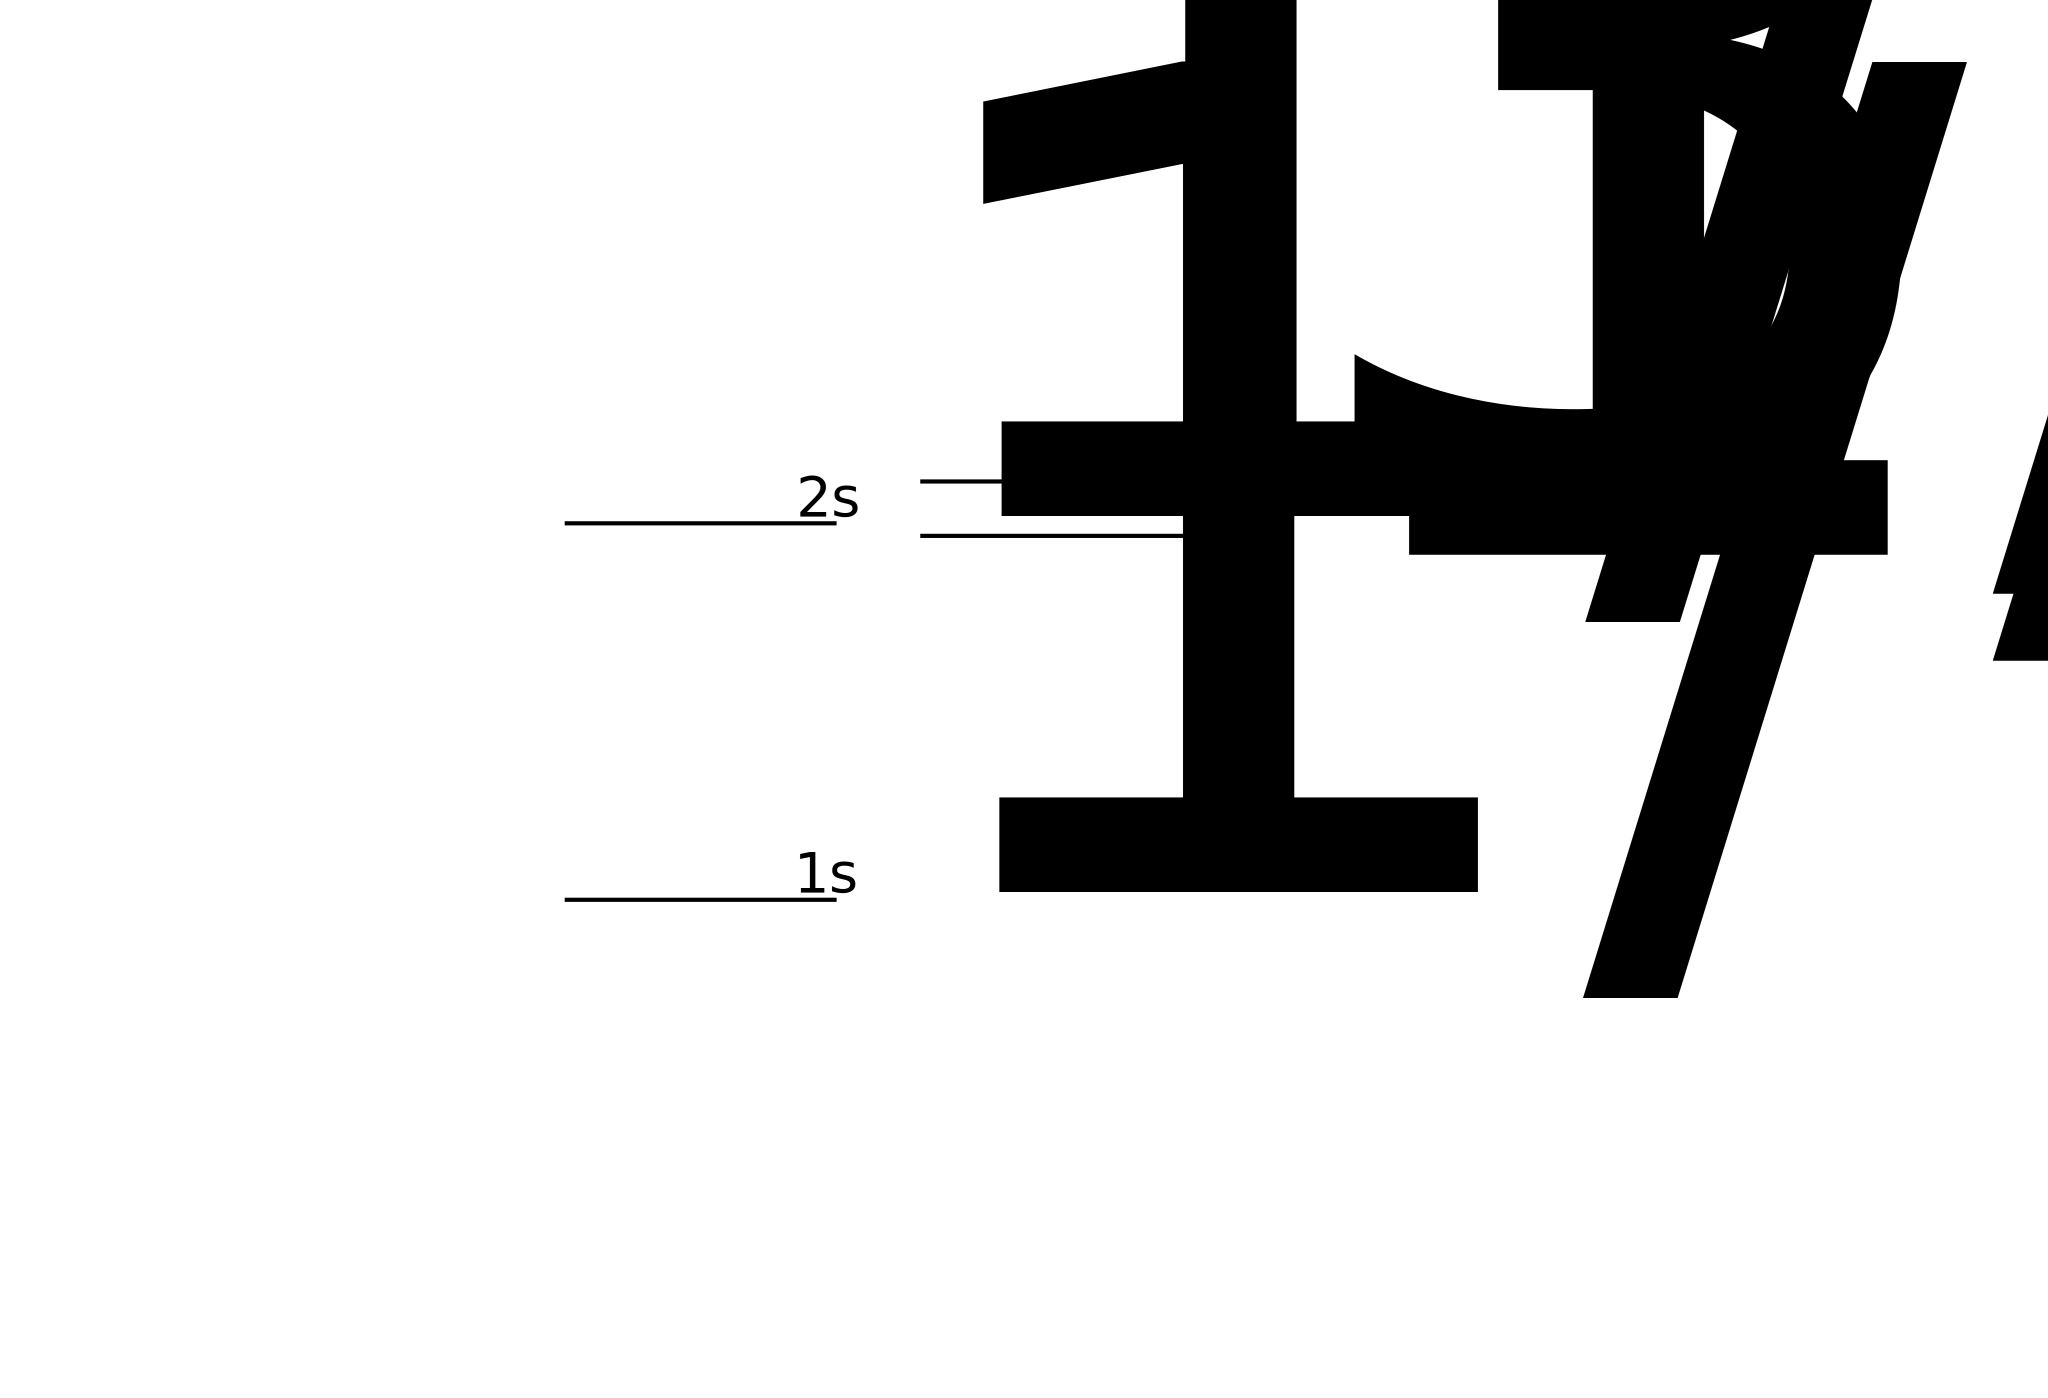
\includegraphics[width=\linewidth]{figs/Hydrogen-Espectrum}
		Спектр нижних уровней атома водорода с учетом лэмбовского сдвига.
	}
	\end{columns}

}

\frame{
	\frametitle{Эффект Казимира}
	% Казимир впервые показал на примере влияние нулевой энергии вакуума на тела
	% Он рассматривал разницу в энергии вакуума, вносимую присутствием идеально проводящих пластин. 
	% Поскольку гамильтониан, содержащий поле фотонов, приводится к интегралу по бесконечному числу гармонических осцилляторов, энергия вакуума выражается суммой аш омега пополам. Рассмотрим куб с достаточно большой стороной эль и ситуацию, когда грани этого куба оказвыаются на расстоянии дэ много меньше ль. Граничные условия с идеальными проводниками дают вот такие значения волнового вектора. 
	% В результате для энергии взаимодействия, то есть разности энергий системы при перемещении пластины, получается такая формула. Этот ряд, естественно, как это всегда бывает с квантовой теорией поля, расходится. 
	% К счастью, для чисел эн находятся физические ограничения. Никакая реальная поверхность не является препятствием для влон чрезвычайно большой частоты. Поэтому нужно просто отрезать ряд для больших волновых векторов. 
	% несмотря на большое единица на дэ квадрат в первой сумме, во второй сумме гораздо больше слагаемых. И это является определяющим при расчетах, энергия взаимодействия оказывается отрицательной. Пластинам выгодно сблизиться. 
	% на пальцах взятие этих сумм можно проиллюстрировать так: Большее значение ль разрешает большему числу волновых векторов участвовать в сумме, а значит при уменьшении ль сумма уменьшается. 
	\centering
	\includegraphics[width=.9\linewidth]{figs/Casimir-cubes}
	\small
	$$
	E_\text{вак.} = \sum\limits_\vec{k} \frac{\hbar\omega(\vec{k})}{2},
	\quad
	\omega(\vec{k}) = |\vec{k}|c,
	\quad
	\vec{k} = \left(\frac{\pi\,n_x}{L_x},\ \frac{\pi\,n_y}{L_y},\ \frac{\pi\,n_z}{L_z}\right)
	$$
	$$
	\Delta E = \frac{\hbar c}{2}\sum\limits_{n_x, n_y, n_z} \left(
	\sqrt{\frac{\pi^2}{L^2}\,n_x^2 + \frac{\pi^2}{L^2}\,n_y^2 + \frac{\pi^2}{d^2}\,n_z^2} \ - \ 
	\sqrt{\frac{\pi^2}{L^2}\,n_x^2 + \frac{\pi^2}{L^2}\,n_y^2 + \frac{\pi^2}{L^2}\,n_z^2}
	\right)
	$$
	$$
	\Delta E = \frac{\hbar c}{2}\sum\limits_{n_x, n_y}\left(
	\sum\limits_{n_z=1}^{\Lambda d/\pi} \sqrt{\frac{\pi^2\,(n_x^2 + n_y^2)}{L^2} + \frac{\pi^2}{d^2}\,n_z^2} \ - \ 
	\sum\limits_{n_z=1}^{\Lambda L/\pi} \sqrt{\frac{\pi^2\,(n_x^2 + n_y^2)}{L^2} + \frac{\pi^2}{L^2}\,n_z^2}
	\right)
	$$
}

\frame{
	\frametitle{Эффект Казимира}
	% Полезно разобрать еще один способ получения сил Казимира. Каждая волна оказывает давление на пластину. Чем меньше расстояние между пластинами, тем меньше волн существует, тем меньше пластины расталкиваются. 
	% Однако, снаружи пространство особо ничем не ограничено, волн в нем может существовать намного больше, чем между. То есть имеется сравнительно сильное давление снаружи на пластины, которое их сдавливает. 
	% В результате они слипаются. 
	% Это рассуждение верно, пока нет необходимости учитывать структуру материала и подобные тонкие вещи
	% На практике это играет очень большую отрицательную роль, поскольку детали наномеханизмов просто слипаются в комок
	% Однако существуют системы, в которых эффект казимира приводит к расталкивающей силе. Например, шар расталкивается флуктуациями (забавный случай)
	\centering
	\vfill
	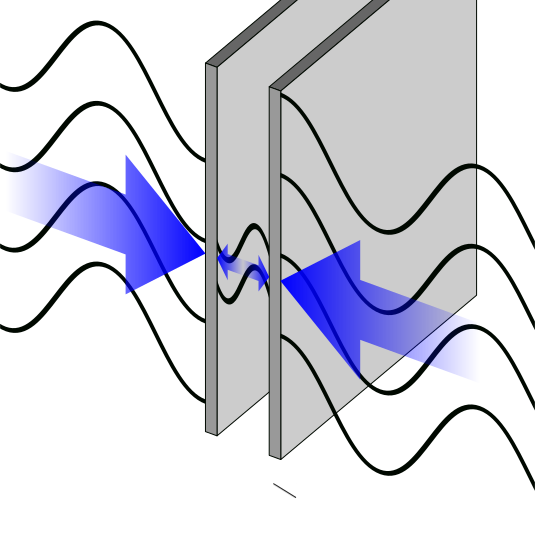
\includegraphics[width=.6\linewidth]{figs/Casimir-plates}

}

\frame{
	\frametitle{Отталкивающие силы Казимира}
	% Их поиск сейчас очень активно ведется, потому что во-первых человечество все же хочет пользоваться наномеханизмами, а во-вторых уж очень привлекательной кажется идея механизмов без прямого соприкосновения, это существенно уменьшает трение 
	% Экспериментально отталкивание наблюдалось лишь в одной конфигурации, между двумя диэлектриками в среде с промежуточной диэлектрической проницаемостью. 
	% Теоретически были обнаружены в системах с идеальными электрическими и магнитными проводниками, метаматериалами, и, что более удачно, например, с эллиптической частицей и плоскостью с дыркой, а также между анизатропно поляризуемыми атомами и различными поверхностями. 
	% Еще однин удачный пример -- в хиральном веществе между проводниками, в присутствии магнитного поля. Приятность этого результата в том, что можно манипулировать силой с помощью внешнего поля, и еще что все точки равновесия устойчивы. 
	\centering
	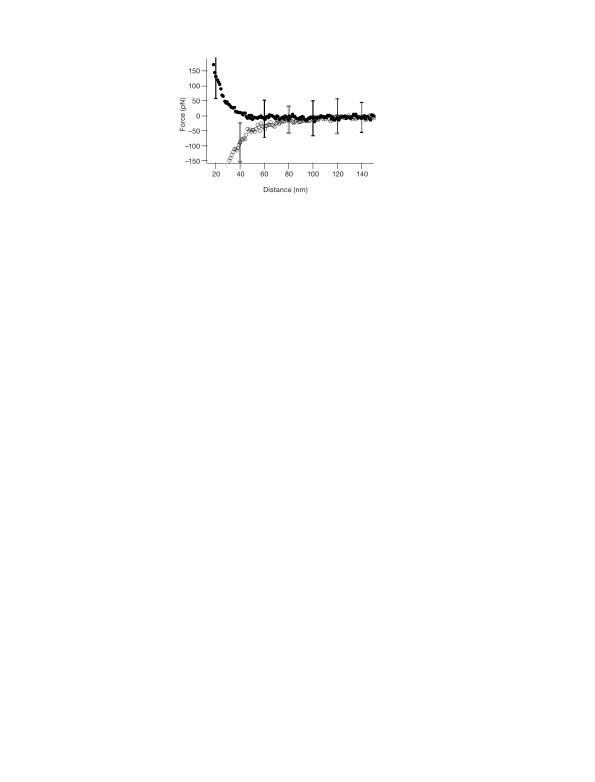
\includegraphics[width=.48\linewidth]{figs/Repulsive-graph}
	\hfill
	\includegraphics[width=.48\linewidth]{figs/Repulsion-aperture}
	\vskip\fill
	\includegraphics[width=.4\linewidth]{figs/Chiral-Casimir}

}

\end{document}




\frame{
	\frametitle{Запаздывание ван-дер-Ваальсовых сил}
	Истинная природа эффекта Казимира скорее не в квантовых флуктуациях, а в релятивистской квантовой силе ван-дер-Ваальса. Попробуй прочитать об этом в Общей теории вдВ сил Лифшица. 

}


\end{document}
